\documentclass[a4paper]{article}

\def\npart {IB}
\def\nterm {Michaelmas}
\def\nyear {2015}
\def\nlecturer {J. M. Evans}
\def\ncourse {Quantum Mechanics}
\def\nlectures {TT.11}
\def\nnotready {}

% Imports
\ifx \nextra \undefined
  \usepackage[pdftex,
    hidelinks,
    pdfauthor={Dexter Chua},
    pdfsubject={Cambridge Maths Notes: Part \npart\ - \ncourse},
    pdftitle={Part \npart\ - \ncourse},
  pdfkeywords={Cambridge Mathematics Maths Math \npart\ \nterm\ \nyear\ \ncourse}]{hyperref}
  \title{Part \npart\ - \ncourse}
\else
  \usepackage[pdftex,
    hidelinks,
    pdfauthor={Dexter Chua},
    pdfsubject={Cambridge Maths Notes: Part \npart\ - \ncourse\ (\nextra)},
    pdftitle={Part \npart\ - \ncourse\ (\nextra)},
  pdfkeywords={Cambridge Mathematics Maths Math \npart\ \nterm\ \nyear\ \ncourse\ \nextra}]{hyperref}

  \title{Part \npart\ - \ncourse \\ {\Large \nextra}}
\fi

\author{Lectured by \nlecturer \\\small Notes taken by Dexter Chua}
\date{\nterm\ \nyear}

\usepackage{alltt}
\usepackage{amsfonts}
\usepackage{amsmath}
\usepackage{amssymb}
\usepackage{amsthm}
\usepackage{booktabs}
\usepackage{caption}
\usepackage{enumitem}
\usepackage{fancyhdr}
\usepackage{graphicx}
\usepackage{mathtools}
\usepackage{microtype}
\usepackage{multirow}
\usepackage{pdflscape}
\usepackage{pgfplots}
\usepackage{siunitx}
\usepackage{tabularx}
\usepackage{tikz}
\usepackage{tkz-euclide}
\usepackage[normalem]{ulem}
\usepackage[all]{xy}

\pgfplotsset{compat=1.12}

\pagestyle{fancyplain}
\lhead{\emph{\nouppercase{\leftmark}}}
\ifx \nextra \undefined
  \rhead{
    \ifnum\thepage=1
    \else
      \npart\ \ncourse
    \fi}
\else
  \rhead{
    \ifnum\thepage=1
    \else
      \npart\ \ncourse\ (\nextra)
    \fi}
\fi
\usetikzlibrary{arrows}
\usetikzlibrary{decorations.markings}
\usetikzlibrary{decorations.pathmorphing}
\usetikzlibrary{positioning}
\usetikzlibrary{fadings}
\usetikzlibrary{intersections}
\usetikzlibrary{cd}

\newcommand*{\Cdot}{\raisebox{-0.25ex}{\scalebox{1.5}{$\cdot$}}}
\newcommand {\pd}[2][ ]{
  \ifx #1 { }
    \frac{\partial}{\partial #2}
  \else
    \frac{\partial^{#1}}{\partial #2^{#1}}
  \fi
}

% Theorems
\theoremstyle{definition}
\newtheorem*{aim}{Aim}
\newtheorem*{axiom}{Axiom}
\newtheorem*{claim}{Claim}
\newtheorem*{cor}{Corollary}
\newtheorem*{defi}{Definition}
\newtheorem*{eg}{Example}
\newtheorem*{fact}{Fact}
\newtheorem*{law}{Law}
\newtheorem*{lemma}{Lemma}
\newtheorem*{notation}{Notation}
\newtheorem*{prop}{Proposition}
\newtheorem*{thm}{Theorem}

\renewcommand{\labelitemi}{--}
\renewcommand{\labelitemii}{$\circ$}
\renewcommand{\labelenumi}{(\roman{*})}

\let\stdsection\section
\renewcommand\section{\newpage\stdsection}

% Strike through
\def\st{\bgroup \ULdepth=-.55ex \ULset}

% Maths symbols
\newcommand{\bra}{\langle}
\newcommand{\ket}{\rangle}

\newcommand{\N}{\mathbb{N}}
\newcommand{\Z}{\mathbb{Z}}
\newcommand{\Q}{\mathbb{Q}}
\renewcommand{\H}{\mathbb{H}}
\newcommand{\R}{\mathbb{R}}
\newcommand{\C}{\mathbb{C}}
\newcommand{\Prob}{\mathbb{P}}
\renewcommand{\P}{\mathbb{P}}
\newcommand{\E}{\mathbb{E}}
\newcommand{\F}{\mathbb{F}}
\newcommand{\cU}{\mathcal{U}}
\newcommand{\RP}{\mathbb{RP}}
\newcommand{\CP}{\mathbb{CP}}

\newcommand{\ph}{\,\cdot\,}

\DeclareMathOperator{\sech}{sech}
\DeclareMathOperator{\cosech}{cosech}
\DeclareMathOperator{\cosec}{cosec}

\DeclareMathOperator{\covol}{covol}
\DeclareMathOperator{\vol}{vol}

\let\Im\relax
\let\Re\relax
\DeclareMathOperator{\Im}{Im}
\DeclareMathOperator{\Re}{Re}
\DeclareMathOperator{\im}{im}
\DeclareMathOperator{\image}{image}
\DeclareMathOperator{\Ann}{Ann}

\DeclareMathOperator*{\res}{res}
\DeclareMathOperator{\Res}{Res}
\DeclareMathOperator{\Ind}{Ind}

\DeclareMathOperator{\tr}{tr}
\DeclareMathOperator{\diag}{diag}
\DeclareMathOperator{\rank}{rank}
\DeclareMathOperator{\card}{card}
\DeclareMathOperator{\spn}{span}
\DeclareMathOperator{\adj}{adj}

\DeclareMathOperator{\erf}{erf}
\DeclareMathOperator{\erfc}{erfc}

\DeclareMathOperator{\ord}{ord}
\DeclareMathOperator{\Sym}{Sym}

\DeclareMathOperator{\sgn}{sgn}
\DeclareMathOperator{\orb}{orb}
\DeclareMathOperator{\stab}{stab}
\DeclareMathOperator{\ccl}{ccl}

\DeclareMathOperator{\lcm}{lcm}
\DeclareMathOperator{\hcf}{hcf}

\DeclareMathOperator{\Int}{Int}
\DeclareMathOperator{\id}{id}

\DeclareMathOperator{\betaD}{beta}
\DeclareMathOperator{\gammaD}{gamma}
\DeclareMathOperator{\Poisson}{Poisson}
\DeclareMathOperator{\binomial}{binomial}
\DeclareMathOperator{\multinomial}{multinomial}
\DeclareMathOperator{\Bernoulli}{Bernoulli}
\DeclareMathOperator{\like}{like}

\DeclareMathOperator{\var}{var}
\DeclareMathOperator{\cov}{cov}
\DeclareMathOperator{\bias}{bias}
\DeclareMathOperator{\mse}{mse}
\DeclareMathOperator{\corr}{corr}

\DeclareMathOperator{\otp}{otp}
\DeclareMathOperator{\dom}{dom}

\DeclareMathOperator{\Root}{Root}
\DeclareMathOperator{\supp}{supp}
\DeclareMathOperator{\rel}{rel}
\DeclareMathOperator{\Hom}{Hom}
\DeclareMathOperator{\Aut}{Aut}
\DeclareMathOperator{\Gal}{Gal}
\DeclareMathOperator{\Mat}{Mat}
\DeclareMathOperator{\End}{End}
\DeclareMathOperator{\Char}{char}
\DeclareMathOperator{\ev}{ev}
\DeclareMathOperator{\St}{St}
\DeclareMathOperator{\Lk}{Lk}
\DeclareMathOperator{\disc}{disc}
\DeclareMathOperator{\Isom}{Isom}
\DeclareMathOperator{\length}{length}
\DeclareMathOperator{\energy}{energy}
\DeclareMathOperator{\area}{area}
\DeclareMathOperator{\Syl}{Syl}
\DeclareMathOperator{\cl}{cl}
\DeclareMathOperator{\fix}{fix}

\newcommand{\GL}{\mathrm{GL}}
\newcommand{\SL}{\mathrm{SL}}
\newcommand{\PGL}{\mathrm{PGL}}
\newcommand{\PSL}{\mathrm{PSL}}
\newcommand{\PSU}{\mathrm{PSU}}
\newcommand{\Or}{\mathrm{O}}
\newcommand{\SO}{\mathrm{SO}}
\newcommand{\U}{\mathrm{U}}
\newcommand{\SU}{\mathrm{SU}}

\renewcommand{\d}{\mathrm{d}}
\newcommand{\D}{\mathrm{D}}

\tikzset{->/.style = {decoration={markings,
                                  mark=at position 1 with {\arrow[scale=2]{latex'}}},
                      postaction={decorate}}}
\tikzset{<-/.style = {decoration={markings,
                                  mark=at position 0 with {\arrowreversed[scale=2]{latex'}}},
                      postaction={decorate}}}
\tikzset{<->/.style = {decoration={markings,
                                   mark=at position 0 with {\arrowreversed[scale=2]{latex'}},
                                   mark=at position 1 with {\arrow[scale=2]{latex'}}},
                       postaction={decorate}}}
\tikzset{->-/.style = {decoration={markings,
                                   mark=at position #1 with {\arrow[scale=2]{latex'}}},
                       postaction={decorate}}}
\tikzset{-<-/.style = {decoration={markings,
                                   mark=at position #1 with {\arrowreversed[scale=2]{latex'}}},
                       postaction={decorate}}}

\tikzset{circ/.style = {fill, circle, inner sep = 0, minimum size = 3}}
\tikzset{mstate/.style={circle, draw, blue, text=black, minimum width=0.7cm}}

\definecolor{mblue}{rgb}{0.2, 0.3, 0.8}
\definecolor{morange}{rgb}{1, 0.5, 0}
\definecolor{mgreen}{rgb}{0.1, 0.4, 0.2}
\definecolor{mred}{rgb}{0.5, 0, 0}

\def\drawcirculararc(#1,#2)(#3,#4)(#5,#6){%
    \pgfmathsetmacro\cA{(#1*#1+#2*#2-#3*#3-#4*#4)/2}%
    \pgfmathsetmacro\cB{(#1*#1+#2*#2-#5*#5-#6*#6)/2}%
    \pgfmathsetmacro\cy{(\cB*(#1-#3)-\cA*(#1-#5))/%
                        ((#2-#6)*(#1-#3)-(#2-#4)*(#1-#5))}%
    \pgfmathsetmacro\cx{(\cA-\cy*(#2-#4))/(#1-#3)}%
    \pgfmathsetmacro\cr{sqrt((#1-\cx)*(#1-\cx)+(#2-\cy)*(#2-\cy))}%
    \pgfmathsetmacro\cA{atan2(#2-\cy,#1-\cx)}%
    \pgfmathsetmacro\cB{atan2(#6-\cy,#5-\cx)}%
    \pgfmathparse{\cB<\cA}%
    \ifnum\pgfmathresult=1
        \pgfmathsetmacro\cB{\cB+360}%
    \fi
    \draw (#1,#2) arc (\cA:\cB:\cr);%
}
\newcommand\getCoord[3]{\newdimen{#1}\newdimen{#2}\pgfextractx{#1}{\pgfpointanchor{#3}{center}}\pgfextracty{#2}{\pgfpointanchor{#3}{center}}}

\def\Xint#1{\mathchoice
   {\XXint\displaystyle\textstyle{#1}}%
   {\XXint\textstyle\scriptstyle{#1}}%
   {\XXint\scriptstyle\scriptscriptstyle{#1}}%
   {\XXint\scriptscriptstyle\scriptscriptstyle{#1}}%
   \!\int}
\def\XXint#1#2#3{{\setbox0=\hbox{$#1{#2#3}{\int}$}
     \vcenter{\hbox{$#2#3$}}\kern-.5\wd0}}
\def\ddashint{\Xint=}
\def\dashint{\Xint-}


\begin{document}
\maketitle
{\small
\noindent\textbf{Physical background}\\
Photoelectric effect. Electrons in atoms and line spectra. Particle diffraction.\hspace*{\fill} [1]

\vspace{10pt}
\noindent\textbf{Schr\"odinger equation and solutions}\\
De Broglie waves. Schr\"odinger equation. Superposition principle. Probability interpretation, density and current.\hspace*{\fill} [2]

\vspace{5pt}
\noindent Stationary states. Free particle, Gaussian wave packet. Motion in 1-dimensional potentials, parity. Potential step, square well and barrier. Harmonic oscillator.\hspace*{\fill} [4]

\vspace{10pt}
\noindent\textbf{Observables and expectation values}\\
Position and momentum operators and expectation values. Canonical commutation relations. Uncertainty principle.\hspace*{\fill} [2]

\vspace{5pt}
\noindent Observables and Hermitian operators. Eigenvalues and eigenfunctions. Formula for expectation value.\hspace*{\fill} [2]

\vspace{10pt}
\noindent\textbf{Hydrogen atom}\\
Spherically symmetric wave functions for spherical well and hydrogen atom.

\vspace{5pt}
\noindent Orbital angular momentum operators. General solution of hydrogen atom.\hspace*{\fill} [5]}

\tableofcontents
\setcounter{section}{-1}
\section{Introduction}
Quantum mechanics (QM) is a radical generalization of classical physics. Profound new features of quantum mechanics include
\begin{enumerate}
  \item \emph{Quantisation} --- Quantities such as energy are often restricted to a discrete set of values, or appear in definite amounts , called \emph{quanta}.
  \item \emph{Wave-particle duality} --- Classical concepts of particles and waves become merged in quantum mechanics. They are different aspects of a single entity. So an electron will no longer be thought of a ``particle'' but an entity that has properties of both particles and waves.
  \item Probability and uncertainty --- Predictions in quantum mechanics involve probability in a fundamental way. This probability does not arise from our lack of knowledge of the system, but is a genuine uncertainty in reality. In particular, there are limits to what we can ask about a physical system, even in principle. For example, the Heisenberg Uncertainty Relation entails that we cannot accurately know the position \emph{and} momentum of a particle.
\end{enumerate}
Quantum mechanics also involves a new fundamental constant $h$ or $\hbar = \frac{h}{2\pi}$. The dimension of this is $[h] = ML^2T^{-1} = [\text{energy}]\times [\text{time}] = [\text{position}] \times [\text{momentum}]$.

We can think of this constant as representing the ``strength'' of quantum effects. Despite having these new profound features, we expect to recover classical physics when we take the limit $\hbar \to 0$.

Historically, there are a few experiments that led to the development of quantum mechanics.
\subsection{Light quanta}
In quantum mechanics, light (or electromagnetic waves) consists of quanta called photons. We can think of them as waves that come in discrete ``packets'' that behave like particles.

In particular, photons behave like particles with energy $E = h \nu = \hbar \omega$, where $\nu$ is the frequency and $\omega = 2\pi \nu$ is the angular frequency. However, we usually don't care about $\nu$ and just call $\omega$ the frequency.

Similarly, the momentum is given by $p = h/\lambda = \hbar k$, where $\lambda$ is the wavelength and $k = 2\pi/\lambda$ is the wave number.

For electromagnetic waves, the speed is $c = \omega/k = \nu\lambda$. This is consistent with the fact that photons are massless particles, since we have
\[
  E = cp,
\]
as entailed by special relativity.

Historically, Planck used the concept of quanta and the energy-frequency relation to derive the spectrum of black body of ``black-body'' radiation that is consistent with experimental results. However, they were not yet sure that light indeed come in quanta. It could have just been a mathematical trick to derive the desired result.

The physical reality of photons was clarified by Einstein in explaining the \emph{photo-electric effect}.

When we shine some light (or electromagnetic radiation $\gamma$) of frequency $\omega$ onto certain metals, this can cause an emission of electrons ($e$). We can measure the maximum kinetic energy $K$ of these electrons.
\begin{center}
  \begin{tikzpicture}
    \draw (-2, 0) -- (2, 0);
    \draw [decorate, decoration={snake}] (-2, 2) -- (0, 0) node [pos = 0.5, anchor=south west] {$\gamma$}; % make curly
    \draw [->] (0, 0) -- (2, 2) node [right] {$e$};
  \end{tikzpicture}
\end{center}
Experiments show that
\begin{enumerate}
  \item The number of electrons emitted depends on the intensity (brightness) of the light, but not the frequency.
  \item The kinetic energy $K$ depends only (linearly) on the frequency but not the intensity.
  \item For $\omega < \omega_0$ (for some critical value $\omega_0$), \emph{no} electrons are emitted at all.
\end{enumerate}
This is hard to understand classically, but is exactly as expected if each electron emitted is due to the impact with a single photon. If $W$ is the energy required to liberate an electron, then we would expect $K = \hbar \omega - W$ by the conservation of energy. We will have no emission if $\omega < \omega_0 = W/\hbar$.

\subsection{Bohr model of the atom}
When we heat atoms up to make them emit light; or shine light at atoms so that they absorb light, we will find that light is emitted and absorbed at very specific frequencies, known as the emission and absorption spectra. This suggests that the inner structure of atoms is discrete.

However, in the classical model, the simplest atom, the hydrogen, consists of an electron with charge $-e$ and mass $m$, orbiting a proton of charge $+e$ and mas $m_p \gg m$ fixed at the origin.

The potential energy is
\[
  V(r) = -\frac{e^2}{4\pi\varepsilon_0}\frac{1}{r}.
\]
This implies that the angular momentum $\mathbf{L}$ is constant, and the energy $E = \frac{1}{2}mv^2 + V(r)$ is constant.

This is not a very satisfactory model for the atom. First of all, it cannot explain the discrete emission and absorption spectra. More importantly, while this model seems like a mini solar system, electromagnetism behave differently from gravitation. To maintain a circular orbit, an acceleration has to be applied onto the electron. Indeed, the force is given by
\[
  F = \frac{mv^2}{r} = \frac{e^2}{4\pi \varepsilon_0}\frac{1}{r^2}.
\]
Accelerating particles emit radiation and lose energy. So according to classical electrodynamics, the electron will just decay into the proton and atoms will implode.

The solution to this problem is to simply declare that this cannot happen. The \emph{Bohr quantization conditions} restricts the classical orbits by saying that the angular momentum can only take values
\[
  L = mrv = n\hbar
\]
for $n = 1, 2, \cdots$. Using these, together with the force equation, we can solve $r$ and $v$ completely for each $n$and obtain
\begin{align*}
  r_n &= \frac{4\pi \varepsilon_0}{me^2}\hbar^2 n^2\\
  v_n &= \frac{e^2}{4\pi \varepsilon_0}\frac{1}{\hbar n}\\
  E_n &= -\frac{1}{2}m\left(\frac{e^2}{4\pi \varepsilon_0 \hbar}\right)^2 \frac{1}{n^2}.
\end{align*}
Now we assume that the electron can make transitions between different energy levels $n$ and $m > n$, accompanied by emission or absorption of a photon of frequency $\omega$ given by
\[
  E = \hbar \omega = E_n - E_m = \frac{1}{2}m \left(\frac{e^2}{4\pi \varepsilon_0 \hbar}\right)^2\left(\frac{1}{n^2} - \frac{1}{m^2}\right).
\]
\begin{center}
  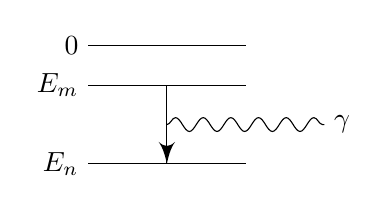
\begin{tikzpicture}
    \draw (-1, 0) node [left] {$0$} -- (1, 0);
    \draw (-1, -0.5) node [left] {$E_m$} -- (1, -0.5);
    \draw (-1, -1.5) node [left] {$E_n$} -- (1, -1.5);
    \draw [->] (0, -0.5) -- (0, -1.5);
    \draw [decorate, decoration={snake}] (0, -1) -- (2, -1) node [right] {$\gamma$};
  \end{tikzpicture}
\end{center}
This model explains a \emph{vast} amount of experimental data. This also gives an estimate of the size of a hydrogen atom:
\[
  r_1 = \left(\frac{4\pi \varepsilon_0}{me^2}\right) \hbar^2 \approx \SI{5.29e-11}{\meter},
\]
known as the \emph{Bohr radius}.

Nevertheless, we would like a better understanding of why angular momentum should be quantized.

\subsection{Matter waves}
The relation
\begin{align*}
  E &= h\nu = \hbar \omega\\
  p &= \frac{h}{\lambda} = \hbar k
\end{align*}
are used to associate particle properties (energy and momentum) to waves. They can also be used the other way round --- to associate wave properties (frequency and wave number) to particles. Moreover, these apply to non-relativistic particles such as electrons (as well as relativistic photons). This $\lambda$ is known as the \emph{de Broglie wavelength}. How does this fit in into our existing model?

Recall that the quantization of the Bohr model requires that
\[
  L = rp = n\hbar.
\]
Using the relations above, this is equivalent to requiring that
\[
  n\lambda = 2\pi r.
\]
This requires that the circumference of the orbit is an integer multiple of the wavelength. This is somewhat the condition we need for a standing wave to form on the circumference. This looks promising as an explanation for the quantization relation.

But in reality, do electrons actually behave like waves? If electrons really are waves, then they should exhibit the usual behaviour of waves, such as diffraction and interference.

We can repeat our favorite double-slit experiment on electrons. We have a sinusoidal wave incident on some barrier with narrow openings as shown:
\begin{center}
  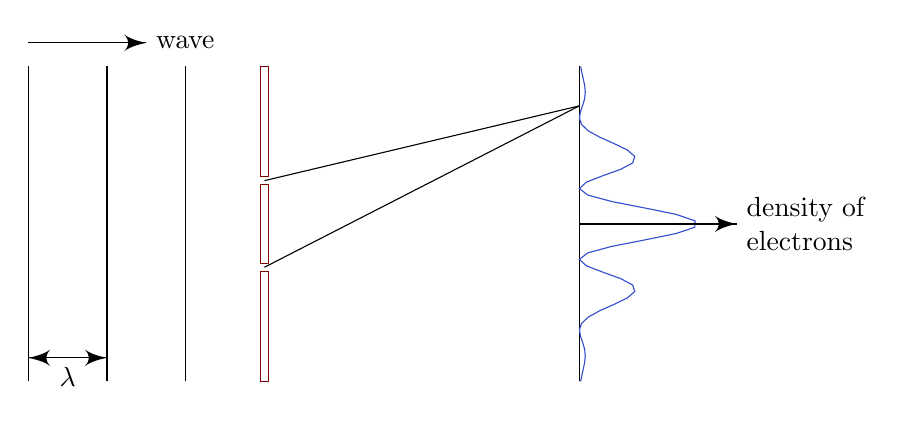
\begin{tikzpicture}
    \draw [mred] (-0.05, -0.5) rectangle (0.05, 0.5);
    \draw [mred] (-0.05, 0.6) rectangle (0.05, 2);
    \draw [mred] (-0.05, -0.6) rectangle (0.05, -2);
    \draw (4, -2) -- (4, 2);

    \foreach \x in {-1, -2, -3} {
      \draw (\x, -2) -- (\x, 2);
    }

    \draw [<->] (-2, -1.7) -- (-3, -1.7) node [below, pos=0.5] {$\lambda$};
    \draw [->] (-3, 2.3) -- (-1.5, 2.3) node [right] {wave};

    \draw (0, 0.55) -- (4, 1.5);
    \draw (0, -0.55) -- (4, 1.5);
    \draw [domain=-2:2,samples=50, mblue] plot ({4 + 1.5 * exp(-\x * \x) * (cos (200 * \x))^2}, \x);
    \draw [->, align=left] (4, 0) -- (6, 0) node [right] {density of\\ electrons};
  \end{tikzpicture}
\end{center}
At different points, Depending on the difference $\delta$ in path length, we may have constructive interference (large amplitude) or destructive interference (no amplitude). In particular, constructive interference occurs if $\delta = n\lambda$, and destructive if $\delta = (n + \frac{1}{2})\lambda$.

Not only does this experiment allow us to verify if something is a wave. We can also figure its wavelength $\lambda$ by experiment.

Practically, the actual experiment for electrons is slightly more complicated. Since the wavelength of an electron is rather small, to obtain the diffraction pattern, we cannot just poke holes in sheets. Instead, we need to use crystals as our diffraction grating. Nevertheless, this shows that electrons do diffract, and the wavelength \emph{is} the de Broglie wavelength.

This also has a conceptual importance. For regular waves, diffraction is something we can make sense of. However, here we are talking about electrons. We know that if we fire many many electrons, the distribution will follow the pattern described above. But what if we just fire a single electron? On \emph{average}, it should still follow the distribution. However, for this individual electron, we cannot know where it will actually land. We can only provide a probability distribution of where it will end up. In quantum mechanics, everything is inherently probabilistic.

As we have seen, quantum mechanics is vastly different from classical mechanics. This is unlike special relativity, where we are just making adjustments to Newtonian mechanics. In fact, in IA Dynamics and Relativity, we just ``derived'' special relativity by assuming the principle of relativity and that the speed of light is independent of the observer. This is not something we can do for quantum mechanics --- what we are going to do is just come up with some theory and then show (or claim) that they agree with experiment.

\section{Wavefunctions and the Schr\"odinger equation}
To begin with, we will concentrate on quantum mechanics in one dimension only.

\subsection{Particle state and probability}
Classically, a point particle in 1 dimension has a definitive position $x$ (and momentum $p$) at each time. In quantum mechanics, a particle has a \emph{state} at each time, specified by a complex-valued \emph{wavefunction} $\psi(x)$.

If $\psi$ is appropriately normalized, then when we measure the position of a particle, we get a result $x$ with probability density function $|\psi(x)|^2$, ie. the probability that the position is found in $[x, x + \delta x]$ (for small $\delta x$) is given by $|\psi(x)|^2 \delta x$. Alternatively, the probability of finding it in $[a, b]$ is given by
\[
  \P(\text{particle position in }[a, b]) = \int_a^b |\psi(x)|^2 \;\d x.
\]
What do we mean by ``appropriately normalized''? From our equation above, we see that we require
\[
  \int_{-\infty}^\infty |\psi(x)|^2\;\d x = 1,
\]
since this is the total probability of finding the particle anywhere at all. This the normalization condition required.

\begin{eg}[Gaussian wavefunction]
  We define
  \[
    \psi(x) = C e^{-\frac{(x - c)^2}{2\alpha}},
  \]
  where $c$ is realm $C$ could be complex.
  \begin{center}
    \begin{tikzpicture}[yscale=1.5]
      \draw (-3, 0) -- (3, 0);
      \draw (0, 1.3) -- (0, 0) node [below] {$c$};
      \draw [domain=-3:3,samples=50, mblue] plot (\x, {exp(-\x * \x)});
    \end{tikzpicture}
  \end{center}
  We have
  \[
    \int_{-\infty}^\infty |\psi(x)|^2 \;\d x = |C|^2 \int_{-\infty}^{\infty}e^{-\frac{(x - c)^2}{\alpha}} \;\d x = |C|^2 (\alpha \pi)^{\frac{1}{2}} = 1.
  \]
  So for normalization, we need to pick $C = (1/\alpha \pi)^{1/4}$ (up to a multiple of $e^{i\theta}$).

  If $\alpha$ is small, then we have a sharp peak around $x = c$. If $\alpha$ is large, it is more spread out.
\end{eg}
While it is nice to have a normalized wavefunction, it is often inconvenient to deal exclusively with normalized wavefunctions, or else we will have a lot of ugly-looking constants floating all around. As a matter of fact, we can always restore normalization at the end of the calculation. So we often don't bother.

If we do not care about normalization, then for any (non-zero) $\lambda$, $\psi(x)$ and $\lambda \psi(x)$ represent the same quantum state (since they give the same probabilities). In practice, we usually refer to either of these as ``the state''.

What we do require, then, is not that the wavefunction is normalized, but \emph{normalizable}, ie.
\[
  \int_{-\infty}^\infty |\psi(x)|^2 \;\d x < \infty.
\]
A characteristic property of quantum mechanics is that if $\psi_1(x)$ and $\psi_2(x)$ are wavefunctions for a particle, then $\psi_1(x) + \psi_2 (x)$ is also a possible particle state (ignoring normalization), provided the result is non-zero. This is the principle of superposition, and arises from the fact that the equations of quantum mechanics are linear.

\begin{eg}[Superposition of Gaussian wavefunctions]
  Take
  \[
    \psi(x) = B\left(\exp\left(\frac{-(x - c)^2}{2\alpha}\right) + \exp\left(-\frac{x^2}{2\beta}\right)\right).
  \]
  Then the resultant distribution would be something like
  \begin{center}
    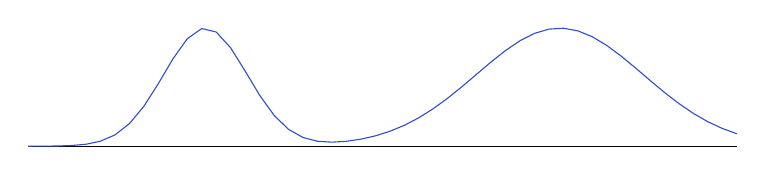
\begin{tikzpicture}[xscale=0.75, yscale=1.5]
      \draw (-3, 0) -- (9, 0);
      \draw [domain=-3:9,samples=50, mblue] plot (\x, {exp(-\x * \x) + exp(-(\x - 6)^2/4)});
    \end{tikzpicture}
  \end{center}
  We choose $B$ so that $\psi$ in a normalized wavefunction for a single particle. Note that this is \emph{not} two particles at two different positions. It is \emph{one} particle that is ``spread out'' at two different positions.
\end{eg}
It is possible that in some cases, the particles in the configuration space may be restricted. For example, we might require $ -\frac{\ell}{2} \leq x \leq \frac{\ell}{2}$ with some boundary conditions at the edges. Then the normalization condition would not be integrating over $(-\infty, \infty)$, but $[-\frac{\ell}{2}, \frac{\ell}{2}]$.

\subsection{Operators}
We know that the square of the wavefunction gives the probability distribution of the \emph{position} of the particle. How about other information such as the momentum and energy? It turns out that all the information about the particle is contained in the wavefunction (which is why we call it the ``state'' of the particle).

We call each property of the particle which we can measure an \emph{observable}. Each observable is represented by an \emph{operator} acting on $\psi(x)$. For example, the position is represented by the operator $\hat{x} = x$. This means that $(\hat{x} \psi)(x) = x\psi(x)$. We can list a few other operators:
\begin{center}
  \begin{tabular}{rll}
    position & $\hat{x} = x$ & $\hat{x} \psi = x\psi(x)$\\
    momentum & $\hat{p} = -i\hbar \frac{\partial}{\partial x}$ & $\hat{p}\psi = -i\hbar \psi'(x)$\\
    energy & $H = \frac{\hat{p}^2}{2m} + V(\hat{x})$ & $H\psi = -\hbar^2 \frac{\partial^2}{\partial x^2}\psi + V(x)\psi(x)$
  \end{tabular}
\end{center}
The final $H$ is called the Hamiltonian, where $m$ is the mass and $V$ is the potential. We see that the Hamiltonian is just the kinetic energy $\frac{p^2}{2m}$ and the potential energy $V$. There will be more insight into why the operators are defined like this in IIC Classical Dynamics and IID Principles of Quantum Mechanics.

Note that we put hats on $\hat{x}$ and $\hat{p}$ to make it explicit that these are operators, as opposed to the classical quantities position and momentum. Otherwise, the definition $\hat{x} = x$ would look silly.

How do these operators relate to the actual physical properties? In general, when we measure an observable, the result is not certain. They are randomly distributed according to some probability distribution, which we will go into full details later.

A \emph{definite} result is obtained if and only if $\psi$ is an eigenstate, or eigenfunction, of the operator. In this case, results of the measurements are the eigenvalue associated. For example, we have
\[
  \hat{p} \psi = p\psi
\]
if and only if $\psi$ is a state with definite momentum $p$. Similarly,
\[
  H\psi = E\psi
\]
if and only if $\psi$ has definite energy $E$.

Here we are starting to see why quantization occurs in quantum mechanics. Since the only possible values of $E$ and $p$ are the eigenvalues, if the operators have a discrete set of eigenvalues, then we can only have discrete values of $p$ and $E$.

\begin{eg}
  Let
  \[
    \psi(x) = Ce^{ikx}.
  \]
  This has a wavelength of $\lambda = 2\pi/k$. This is a momentum eigenstate, since we have
  \[
    \hat{p}\psi = -\hbar \psi' = (\hbar k)\psi.
  \]
  So we know that the momentum eigenvalue is $p = \hbar k$. This looks encouraging!

  Note that if there is no potential, ie. $V = 0$, then
  \[
    H\psi = \frac{\hat{p}^2}{2m}\psi = -\frac{\hbar^2}{2m}\psi'' = \frac{\hbar^2 k^2}{2m}\psi.
  \]
  So the energy eigenvalue is
  \[
    E = \frac{\hbar^2 k^2}{2m}.
  \]
\end{eg}
Note, however, that our wavefunction has $|\psi(x)|^2 = |C|^2$, which is a constant. So this wavefunction is not normalizable on the whole line. However, if we restrict ourselves to some finite domain $-\frac{\ell}{2} \leq x \leq \frac{\ell}{2}$, then we can normalize by picking $C= \frac{1}{\sqrt{\ell}}$.

\begin{eg}
  Consider the Gaussian distribution
  \[
    \psi(x) = C\exp\left(-\frac{x^2}{2\alpha}\right).
  \]
  We get
  \[
    \hat{p}\psi(x) = -i\hbar \psi'(x) \not= p\psi(x)
  \]
  for any number $p$. So this is not an eigenfunction of the momentum.

  However, if we consider the harmonic oscillator with potential
  \[
    V(x) = \frac{1}{2}Kx^2,
  \]
  then this $\psi(x)$ is an eigenfunction of the Hamiltonian operator, provided we picked the right $\alpha$. We have
  \[
    H\psi = -\frac{\hbar^2}{2m}\psi'' + \frac{1}{2}Kx^2 \psi = E\psi
  \]
  when $\alpha^2 = \frac{\hbar^2}{Km}$. Then the energy is $E = \frac{\hbar}{2}\sqrt{\frac{K}{m}}$. This is to be verified on the example sheet.
\end{eg}
Despite being a simple system, the harmonic oscillator is \emph{incredibly} useful in theoretical physics. We will hence solve this completely later.

\begin{defi}[Time-independent Schr\"odinger equation]
  The \emph{time-independent Schr\"odinger equation} is the energy eigenvalue equation
  \[
    H\psi = E\psi,
  \]
  or
  \[
    -\frac{\hbar^2}{2m}\psi'' + V(x) \psi = E\psi.
  \]
\end{defi}
This is in general what determines what the system behaves. In particular, the eigenvalues $E$ are precisely the allowed energy value.

\subsection{Time evolution of wavefunctions}
So far, everything is instantaneous. The wavefunction specifies the state \emph{at a particular time}, and the eigenvalues are the properties of the system \emph{at that particular time}. However, this is quantum \emph{mechanics}, or quantum \emph{dynamics}. We should be looking at how things \emph{change}. We want to know how the wavefunction changes with time. This is what we will get to now.

\subsubsection{Time-dependent Schr\"odinger equation}
We will write $\Psi$ instead of $\psi$ to indicate that we are looking at the time-dependent wavefunction. The evolution of this $\Psi(x, t)$ is described by the time-dependent Schr\"odinger equation.
\begin{defi}[Time-dependent Schr\"odinger equation]
  For a time-dependent wavefunction $\Psi(x, t)$, the \emph{time-dependent Schr\"odinger equation} is
  \[
    i\hbar \frac{\partial \Psi}{\partial t} = H\Psi.\tag{$*$}
  \]
\end{defi}
For a particle in a potential $V(x)$, this can reads
\[
  i\hbar \frac{\partial \Psi}{\partial t} = -\frac{\hbar^2}{2m}\frac{\partial^2 \Psi}{\partial x^2} + V(x) \Psi.
\]
While this looks rather scary, it isn't really that bad. First of all, it is linear. So the sums and multiples of solutions are also solutions. It is also first-order in time. So if we know the wavefunction $\Psi(x, t_0)$ at a particular time $t_0$, then this determines the whole function $\Psi(x, t)$.

This is similar to classical dynamics, where knowing the potential $V$ (and hence the Hamiltonian $H$) completely specifies how the system evolves with time. However, this is in some ways different from classical dynamics. Newton's second law is second-order in time, while this is first-order in time. This is significant since when our equation is first-order in time, then the current state of the wavefunction completely specifies the evolution of the wavefunction in time.

This is since the wavefunction is the \emph{state} of the particle, and not just the ``position''. Instead, we can think of it as capturing the position \emph{and} momentum. Indeed, if we write the equations of classical dynamics in terms of position and momentum, it will be first order in time.

\subsubsection{Stationary states}
Consider a special class of solutions $\Psi(x, t) = T(t) \psi(x)$, where $\Psi(x, 0) = \psi(x)$ (ie. $T(0) = 1$). If $\psi$ satisfies the time-independent Schr\"odinger equation
\[
  H\psi = E\psi,
\]
then it is an energy eigenstate at each fixed $t$, ie.
\[
  H\Psi = E\Psi.
\]
So if we want this $\Psi$ to satisfy the Schr\"odinger equation, we must have
\[
  i\hbar \dot{T} = ET.
\]
The solution is obvious:
\[
  T(t) = \exp\left(-\frac{iEt}{\hbar}\right).
\]
We can write our full solution as
\[
  \Psi(x, t) = \psi(x) \exp\left(-\frac{iEt}{\hbar}\right).
\]
Note that the frequency is $\omega = \frac{E}{\hbar}$. So we recover the Energy-frequency relation we previously had.

\begin{defi}[Stationary state]
  A \emph{stationary state} is a state of the form
  \[
    \Psi(x, t) = \psi(x) \exp\left(-\frac{iEt}{\hbar}\right).
  \]
  where $\psi(x)$ is an eigenfunction of the Hamiltonian with eigenvalue $E$. This term is also sometimes applied to $\psi$ instead.
\end{defi}
For such a state,
\[
  |\Psi(x, t)|^2 = |\psi(x)|^2,
\]
which is independent of time.

\subsubsection{Conservation of probability}
Consider a general $\Psi(x, t)$ obeying the time-dependent Schr\"odinger equation.

\begin{prop}
  The probability density
  \[
    P(x, t) = |\Psi(x, t)|^2
  \]
  obeys a conservation equation
  \[
    \frac{\partial P}{\partial t} = - \frac{\partial j}{\partial x},
  \]
  where
  \[
    j(x, t) = -\frac{i\hbar}{2m} (\Psi^*\Psi' - \Psi'^* \Psi)
  \]
  is the \emph{probability current}.
\end{prop}
Since $\Psi^* \Psi'$ is the complex conjugate of $\Psi'^* \Psi$, we know that $\Psi^*\Psi' - \Psi'^* \Psi$ is imaginary. So multiplying by $i$ ensures that $j(x, t)$ is real.

\begin{proof}
  It is straightforward from the Schr\"odinger equation and its complex conjugate. We have
  \begin{align*}
    \frac{\partial P}{\partial t} &= \Psi^* \frac{\partial \Psi}{\partial t} + \frac{\partial \Psi*}{\partial t} \Psi\\
    &= \Psi^* \frac{i\hbar }{2m}\Psi'' - \frac{i\hbar}{2m}\Psi''^* \Psi\\
    \intertext{where the two $V$ terms cancel each other out, assuming $V$ is real}
    &= -\frac{\partial j}{\partial x}.
  \end{align*}
\end{proof}
The important thing here is not the specific form of $j$, but that $\frac{\partial P}{\partial t}$ can be written as the space derivative of some quantity. This implies that the probability that we find the particle in $[a, b]$ at fixed time $t$ changes as
\[
  \frac{\d}{\d t}\int_a^b |\Psi(x, t)|^2 \;\d x = \int_a^b -\frac{\partial j}{\partial x}(x, t)\;\d x = j(a, t) - j(b, t).
\]
We can think of the final term as the probability current getting in and out of the interval at the boundary.

In particular, consider a normalizable state with $\Psi, \Psi', j \to 0$ as $x \to \pm\infty$ for fixed $t$. Taking $a \to -\infty$ and $b\to +\infty$, we have
\[
  \frac{\d}{\d t}\int_{-\infty}^\infty |\Psi(x, t)|^2 \;\d x = 0.
\]
What does this tell us? This tells us that if $\Psi(x, 0)$ is normalized, $\Psi(x, t)$ is normalized for all $t$. We know that for each fixed $t$, $|\Psi(x, t)|^2$ is a probability distribution. So what this really says is that the probability interpretation is consistent with the time evolution.

\section{Some examples in one dimension}
\subsection{Introduction}
In general, we are going to consider the energy eigenvalue problem for a particle in 1 dimension in a potential $V(x)$, ie.
\[
  H\psi = -\frac{\hbar^2}{2m}\Psi'' + V(x) \psi = E\psi.
\]
In other words, we want to find the allowed energy eigenvalues.

This is a hard problem in general. However, we can consider the really easy case where $V(X) = U$, where $U$ is a constant. Then we can easily write down solutions.

If $U > E$, then the Schr\"odinger equation is equivalent to
\[
  \psi'' - \kappa^2 \psi = 0,
\]
where $\kappa$ is such that $U - E = \frac{\hbar^2 \kappa^2}{2m}$. We take wlog $\kappa > 0$. The solution is then
\[
  \psi = Ae^{\kappa x} + Be^{-\kappa x}.
\]
On the other hand, if $U < E$, then the Schr\"odinger equation says
\[
  \psi + k^2 \psi = 0,
\]
where $k$ is picked such that $E - U = \frac{\hbar^2 k^2}{2m}$. The solutions are
\[
  \psi = Ae^{ikx} + Be^{ikx}.
\]
Note that these new constants are merely there to simplify our equations. They generally need not have physical meanings.

Now why are we interested in cases where the potential is constant? Wouldn't that be just equivalent to a free particle? The significance is that we can use these to study piecewise flat potentials such as steps, wells and barriers.
\begin{center}
  \begin{tikzpicture}
    \begin{scope}
      \draw [->] (-1.5, 0) -- (1.5, 0) node [right] {$x$};
      \draw [->] (0, -0.5) -- (0, 1.5) node [above] {$V$};
      \draw [mred, semithick] (-1.5, 0) -- (0, 0) -- (0, 1) -- (1, 1);
    \end{scope}

    \begin{scope}[shift={(4, 0)}]
      \draw [->] (-1.5, 0) -- (1.5, 0) node [right] {$x$};
      \draw [->] (0, -0.5) -- (0, 1.5) node [above] {$V$};
      \draw [mred, semithick] (-1.5, 1) -- (-0.5, 1) -- (-0.5, 0) -- (0.5, 0) -- (0.5, 1) -- (1.5, 1);
    \end{scope}

    \begin{scope}[shift={(8, 0)}]
      \draw [->] (-1.5, 0) -- (1.5, 0) node [right] {$x$};
      \draw [->] (0, -0.5) -- (0, 1.5) node [above] {$V$};
      \draw [mred, semithick] (-1.5, 0) -- (-0.5, 0) -- (-0.5, 1) -- (0.5, 1) -- (0.5, 0) -- (1.5, 0);
    \end{scope}
  \end{tikzpicture}
\end{center}
Here a finite discontinuity in $V$ is allowed. In this case, we can have $\psi, \psi'$ continuous and $\psi''$ discontinuous. Then the discontinuity of $\psi''$ cancels that of $V$, and the Schr\"odinger equation holds everywhere.

In this chapter, we will seek normalizable solutions with
\[
  \int_{-\infty}^\infty |\psi(x)|^2 \;\d x.
\]
This requires that $\psi(x) \to 0$ as $x \to \pm\infty$. We see that for the segments and the end, we want to have decaying exponentials $e^{-\kappa x}$ instead of oscillating exponentials $e^{-ikx}$.

\subsection{Infinite well --- Particle in a box}
Our potential is as follows:
\begin{center}
  \begin{tikzpicture}
    \draw [->] (-2.5, 0) -- (2.5, 0) node [right] {$x$};
    \draw [->] (0, -0.5) -- (0, 2) node [above] {$V$};
    \draw [mred, semithick, ->] (-1.5, 0) node [below] {$-a$} -- (-1.5, 2);
    \draw [mred, semithick, ->] (1.5, 0) node [below] {$a$} -- (1.5, 2);
    \draw [mred, semithick] (-1.5, 0) -- (1.5, 0);
  \end{tikzpicture}
\end{center}
\[
  V(x) =
  \begin{cases}
    0 & |x| \leq a\\
    \infty & |x| > a.
  \end{cases}
\]
We require $\psi = 0$ for $|x| > a$ and $\psi$ continuous at $x = \pm a$. Within $|x| < a$, the Schr\"odinger equation is
\[
  -\frac{\hbar^2}{2m}\psi'' = E\psi.
\]
We simplify this to become
\[
  \psi'' + k^2 \psi = 0,
\]
where
\[
  E = \frac{\hbar^2 k^2}{2m}.
\]
Here, instead of working with the complex exponentials, we use $\sin$ and $\cos$ since we know well when these vanish. The general solution is thus
\[
  \psi = A\cos kx + B\sin kx.
\]
Our boundary conditions require that $\psi$ vanishes at $x = \pm a$. So we need
\[
  A \cos ka \pm B\sin ka = 0.
\]
In other words, we require
\[
  A\cos ka = B\sin ka = 0.
\]
Since $\sin ka$ and $\cos ka$ cannot be simultaneously $0$, either $A = 0$ or $B = 0$. So the two possibilities are
\begin{enumerate}
  \item $B = 0$ and $ka = n\pi/2$ with $n = 1, 3, \cdots$
  \item $A = 0$ and $ka = n\pi/2$ with $n = 2, 4, \cdots$
\end{enumerate}
Hence the allowed energy levels are
\[
  E_n = \frac{\hbar^2 \pi^2}{8ma^2} n^2,
\]
where $n = 1, 2, \cdots$, and the wavefunctions are
\[
  \psi_n(x) = \left(\frac{1}{a}\right)^{\frac{1}{2}}
  \begin{cases}
    \cos \frac{n\pi x}{2a} & n\text{ odd}\\
    \sin \frac{n\pi x}{2a} & n\text{ even}
  \end{cases}.
\]
These are normalized with $\int_{-a}^a |\psi_n(x)|^2 \;\d x$.
\begin{center}
  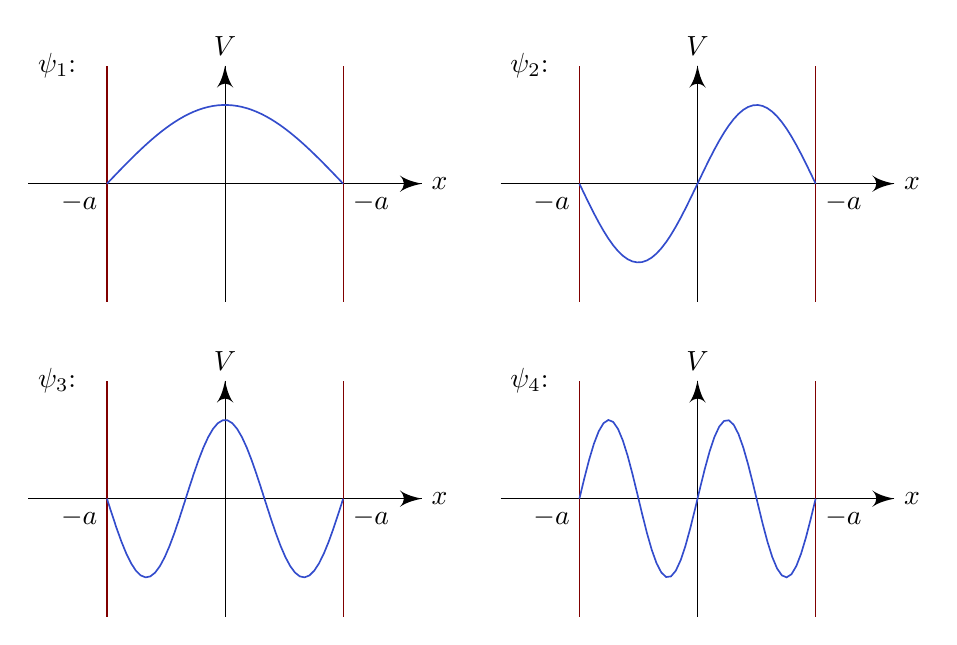
\begin{tikzpicture}
    \begin{scope}
      \node [right] at (-2.5, 1.5) {$\psi_1$:};
      \draw [->] (-2.5, 0) -- (2.5, 0) node [right] {$x$};
      \draw [->] (0, -1.5) -- (0, 1.5) node [above] {$V$};
      \node [anchor = north east] at (-1.5, 0) {$-a$};
      \node [anchor = north west] at (1.5, 0) {$-a$};
      \draw [mred] (-1.5, -1.5) -- (-1.5, 1.5);
      \draw [mred] (1.5, -1.5) -- (1.5, 1.5);

      \draw [mblue, semithick, domain=-1.5:1.5, samples=50] plot (\x, {cos (60 * \x)});
    \end{scope}

    \begin{scope}[shift={(6, 0)}]
      \node [right] at (-2.5, 1.5) {$\psi_2$:};
      \draw [->] (-2.5, 0) -- (2.5, 0) node [right] {$x$};
      \draw [->] (0, -1.5) -- (0, 1.5) node [above] {$V$};
      \node [anchor = north east] at (-1.5, 0) {$-a$};
      \node [anchor = north west] at (1.5, 0) {$-a$};
      \draw [mred] (-1.5, -1.5) -- (-1.5, 1.5);
      \draw [mred] (1.5, -1.5) -- (1.5, 1.5);

      \draw [mblue, semithick, domain=-1.5:1.5, samples=50] plot (\x, {sin (120 * \x)});
    \end{scope}

    \begin{scope}[shift={(0, -4)}]
      \node [right] at (-2.5, 1.5) {$\psi_3$:};
      \draw [->] (-2.5, 0) -- (2.5, 0) node [right] {$x$};
      \draw [->] (0, -1.5) -- (0, 1.5) node [above] {$V$};
      \node [anchor = north east] at (-1.5, 0) {$-a$};
      \node [anchor = north west] at (1.5, 0) {$-a$};
      \draw [mred] (-1.5, -1.5) -- (-1.5, 1.5);
      \draw [mred] (1.5, -1.5) -- (1.5, 1.5);

      \draw [mblue, semithick, domain=-1.5:1.5, samples=50] plot (\x, {cos (180 * \x)});
    \end{scope}

    \begin{scope}[shift={(6, -4)}]
      \node [right] at (-2.5, 1.5) {$\psi_4$:};
      \draw [->] (-2.5, 0) -- (2.5, 0) node [right] {$x$};
      \draw [->] (0, -1.5) -- (0, 1.5) node [above] {$V$};
      \node [anchor = north east] at (-1.5, 0) {$-a$};
      \node [anchor = north west] at (1.5, 0) {$-a$};
      \draw [mred] (-1.5, -1.5) -- (-1.5, 1.5);
      \draw [mred] (1.5, -1.5) -- (1.5, 1.5);

      \draw [mblue, semithick, domain=-1.5:1.5, samples=50] plot (\x, {sin (240 * \x)});
    \end{scope}
  \end{tikzpicture}
\end{center}
This was a rather simple and nice example. We have an infinite well, and the particle is well-contained inside the box.

Note that $\psi_n(-x) = (-1)^{n + 1}\psi_n(x)$. We will see that this is a general feature of energy eigenfunctions of a symmetric potential. This is known as \emph{parity}.
\subsection{Parity}
Consider the Schr\"odinger equation for a particle of mass $m$
\[
  H\psi = -\frac{\hbar^2}{2m}\psi'' + V(x) \psi = E\psi.
\]
with potential
\[
  V(x) = V(-x).
\]
By changing variables $x \to -x$, we see that $\psi(x)$ is an eigenfunction of $H$ with energy $E$ if and only if $\psi(-x)$ is an eigenfunction of $H$ with energy $E$. There are two possibilities:
\begin{enumerate}
  \item If $\psi(x)$ and $\psi(-x)$ represent the same quantum state, this can only happen if $\psi(-x) = \eta \psi(x)$ for some constant $\eta$. Since this is true for all $x$, we can do this twice and get
    \[
      \psi(x) = \eta \psi(-x) = \eta^2 \psi(x).
    \]
    So we get that $\eta = \pm 1$ and $\psi(-x) = \pm \psi(x)$. We call $\eta$ the \emph{parity}, and say $\psi$ has even/odd parity if $\eta$ is $+1/-1$ respectively.

    For example, in our particle in a box, our states $\psi_n$ have parity $(-1)^{n + 1}$.
  \item If $\psi(x)$ and $\psi(-x)$ represent different quantum states, then we can still take linear combinations
    \[
      \psi_\pm (x) = \alpha(\psi(x) \pm \psi(-x)),
    \]
    and these are also eigenstates with energy eigenvalue $E$, where $\alpha$ is for normalization. Then by construction, $\psi_\pm (-x) = \pm \psi_\pm(x)$ and have parity $\eta = \pm 1$.
\end{enumerate}
Hence, if we are given a potential with reflective symmetry $V(-x) = V(x)$, then we can restrict our attention and just look for solutions with definite parity.
\subsection{Potential Well}
We will consider a potential that looks like this:
\begin{center}
  \begin{tikzpicture}[scale=1.5]
    \draw [->] (-1.5, 0) -- (1.5, 0) node [right] {$x$};
    \draw [->] (0, -1.5) -- (0, 0.5) node [above] {$V$};
    \draw [mred, semithick] (-1.5, 0) -- (-0.5, 0) -- (-0.5, -1) node [below] {$-a$} -- (0.5, -1) node [below] {$a$} -- (0.5, 0) -- (1.5, 0);

    \draw [dashed] (0.5, -1) -- (1.5, -1) node [right] {$-U$};
  \end{tikzpicture}
\end{center}
The potential is given by
\[
  V(x) =
  \begin{cases}
    -U & |x| < a\\
    0 & |x| \geq a
  \end{cases}
\]
for some constant $U > 0$. Classically, this is not very interesting. If the energy $E < 0$, then the particle is contained in the well. Otherwise it is free to move around. However, in quantum mechanics, this is much more interesting.

We want to seek energy levels for a particle of mass $m$, defined by the Schr\"odinger equation
\[
  H\psi = -\frac{\hbar^2}{2m}\psi'' + V(x) \psi = E\psi.
\]
For energies in the range
\[
  -U < E < 0,
\]
we set
\[
  U + E = \frac{\hbar^2 k^2}{2m} > 0,\quad E = -\frac{\hbar^2 \kappa^2}{2m},
\]
where $k, \kappa > 0$ are new real constants. Note that these coefficients are not independent, since $U$ is given and fixed. Sing we have
\[
  k^2 + \kappa^2 = \frac{2mU}{\hbar^2}.
\]
Using these constants, the Schr\"odinger equation becomes
\[
  \begin{cases}
    \psi'' + k^2 \psi = 0 & |x| < a\\
    \psi'' - \kappa^2 \psi = 0 & |x| > a.
  \end{cases}
\]
As we previously said, we want the Schr\"odinger equation to hold even at the discontinuities. So we need $\psi$ and $\psi'$ to be continuous at $x = \pm a$.

We first consider the even parity solutions $\psi(-x) = \psi(x)$. We can write our solution as
\[
  \psi =
  \begin{cases}
    A \cos kx & |x| < a\\
    B e^{-\kappa |x|}  & |x| > a\\
  \end{cases}
\]
We match $\psi$ and $\psi'$ at $x = a$. So we need
\begin{align*}
  A\cos ka &= Be^{-\kappa a}\\
  -Ak\sin ka &= -\kappa Be^{-\kappa a}.
\end{align*}
By parity, there is no additional information from $x = -a$.

We can divide the equations to obtain
\[
  k \tan ka = \kappa.
\]
this is still not something we can solve easily. To find when solutions exist, it is convenient to introduce
\[
  \xi = ak, \quad \eta = a\kappa,
\]
where these two constants are dimensionless and positive. Note that this $\eta$ has nothing to do with parity. It's just that we have run out of letters to use. Hence the solution we need are solutions to
\[
  \eta = \xi \tan \xi.
\]
Also, our initial conditions on $k$ and $\kappa$ require
\[
  \xi^2 + \eta^2  = \frac{2ma^2 U}{\hbar^2}.
\]
We can look for solutions by plotting these two equations. We first plot the curve $\eta = \xi \tan \xi$:
\begin{center}
  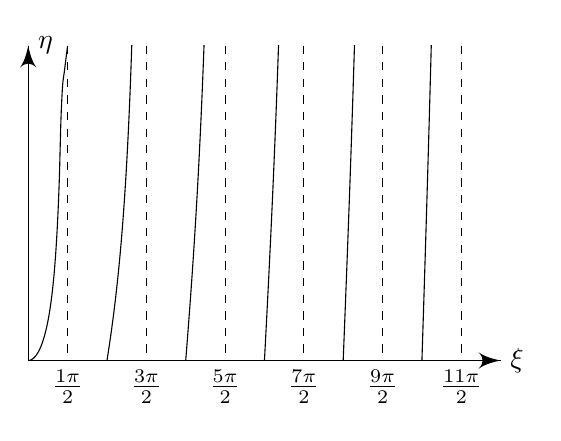
\begin{tikzpicture}
    \draw [->] (0, 0) -- (6, 0) node [right] {$\xi$};
    \draw [->] (0, 0) -- (0, 4) node [right] {$\eta$};
    \begin{scope}[yscale=2]
      \clip (0, 0) rectangle (6, 2);
      \foreach \a in {0,1,...,5} {
        \pgfmathsetmacro\b{\a + 0.499};
        \draw [domain=\a:\b] plot [smooth] (\x, {\x * min(4, tan(180*\x))});
      }
    \end{scope}
    \foreach \a in {0,1,...,5} {
        \pgfmathsetmacro\n{\a * 2 + 1};
      \draw [dashed] (\a + 0.5, 4) -- (\a + 0.5, 0) node [below] {$\frac{\pgfmathprintnumber{\n} \pi}{2}$};
    }
  \end{tikzpicture}
\end{center}
The other equation is the equation of a circle. Depending on the size of the constant $2ma^2 U/\hbar^2$, there will be a different number of points of intersections.
\begin{center}
  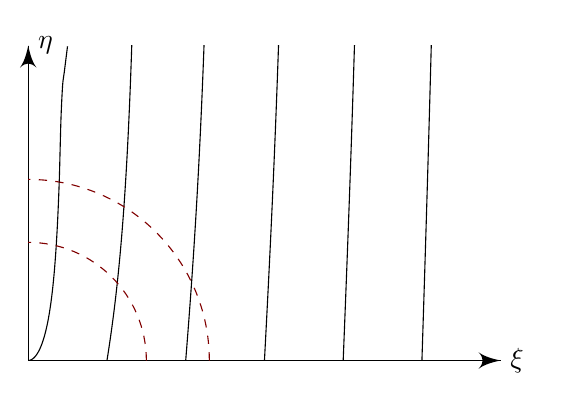
\begin{tikzpicture}
    \draw [->] (0, 0) -- (6, 0) node [right] {$\xi$};
    \draw [->] (0, 0) -- (0, 4) node [right] {$\eta$};
    \begin{scope}[yscale=2]
      \clip (0, 0) rectangle (6, 2);
      \foreach \a in {0,1,...,5} {
        \pgfmathsetmacro\b{\a + 0.499};
        \draw [domain=\a:\b] plot [smooth] (\x, {\x * min(4, tan(180*\x))});
      }
    \end{scope}
    \draw [mred, dashed] (2.3, 0) arc (0:90:2.3);
    \draw [mred, dashed] (1.5, 0) arc (0:90:1.5);
  \end{tikzpicture}
\end{center}
So there will be a different number of solutions depending on the value of $2ma^2 U/\hbar^2$. In particular, if
\[
  (n - 1)\pi < \left(\frac{2mUa^2}{\hbar^2}\right)^{1/2} < n\pi,
\]
then we have exactly $n$ even parity solutions (for $n \geq 1$).

We can do exactly the same thing for odd parity eigenstates\ldots on Example Sheet 1.

For $E > 0$ or $E < -U$, we will end up finding non-normalizable solutions. What is more interesting, though is to look at the solutions we have now. We can compare what we've got with what we would expect classically.

Classically, any value of $E$ in the range $-U < E < 0$ is allowed, and the motion is deeply uninteresting. The particle just goes back and forth inside the well, and is \emph{strictly confined} in $-a \leq x \leq a$.

Quantum mechanically, there is just a discrete, \emph{finite} set of allowed energies. What is more surprising is that while $\psi$ decays exponentially outside the well, it is non-zero! This means there is in theory a non-zero probability of finding the particle outside the well! We call these particles \emph{bound} in the potential, but in fact there is a non-zero probability of finding the particle outside the well.

\subsection{The harmonic oscillator}
So far in our examples, the quantization (mathematically) comes from us requiring continuity at the boundaries. In the harmonic oscillator, it arises in a different way.
\begin{center}
  \begin{tikzpicture}[scale=1.5]
    \draw [->] (-1.5, 0) -- (1.5, 0) node [right] {$x$};
    \draw [->] (0, -0.5) -- (0, 1.5) node [above] {$V$};
    \draw [mred, semithick] (-1, 1.5) parabola bend (0, 0) (1, 1.5);
  \end{tikzpicture}
\end{center}
This is a harmonic oscillator of mass $m$ with
\[
  V(x) = \frac{1}{2}m\omega^2 x^2.
\]
Classically, this has a motion of $x = A \cos \omega (t - t_0)$.

This is a \emph{really} important example. First of all, we can solve it, which is a good thing. More importantly, any smooth potential can be approximated by a harmonic oscillator near an equilibrium $x_0$, since
\[
  V(x) = V(x_0) + \frac{1}{2}V''(x_0)(x - x_0)^2 + \cdots.
\]
Systems with many degrees like crystals can also be treated as collections of independent oscillators by considering the normal modes. If we apply this to the electromagnetic field, we get photons! So it is very important to understand the quantum mechanical oscillator.

We are going to seek all normalizable solutions to the time-independent Schr\"odinger equation
\[
  H\psi = -\frac{\hbar^2}{2m}\psi'' + \frac{1}{2}m\omega^2 x^2 \psi = E\psi.
\]
So simplify constants, we define
\[
  y = \left(\frac{m\omega}{\hbar}\right)^{\frac{1}{2}}x,\quad \mathcal{E} = \frac{2E}{\hbar \omega},
\]
both of which is dimensionless. Then we are left with
\[
  -\frac{\d^2 \psi}{\d y^2} + y^2\psi = \mathcal{E} \psi.
\]
We can consider the behaviour for $y^2 \gg \mathcal{E}$. For large $y$, the $y^2 \psi$ term will be large, and so we want the $\psi''$ term to offset it. We might want to try the Gaussian $e^{-y^2/2}$, and when we differentiate it twice, we would have brought down a factor of $y^2$. So we can wlog set
\[
  \psi = f(y) e^{-\frac{1}{2}y^2}.
\]
Then the Schr\"odinger equation gives
\[
  \frac{\d^2 f}{\d y^2} - 2y\frac{\d f}{\d y} + (\mathcal{E} - 1) = 0.
\]
This is known as \emph{Hermite's equation}. We try a series solution
\[
  f(y) = \sum_{r \geq 0} a_r y^r,
\]
and substitute in to get
\[
  \sum_{r \geq 0} \big( (r + 2)(r + 1)a_{n + 2} + (\mathcal{E} - 1 - 2r)a_r\big) y^r = 0.
\]
This holds if and only if
\[
  a_{r + 2} = \frac{2 r + 1 - \mathcal{E}}{(r + 2)(r + 1)} a_r.\quad r \geq 0.
\]
We can choose $a_0$ and $a_1$ independently, and can get two linearly independent solutions. Each solution involves either all even or all odd powers.

However, we have a problem. We want normalizable solutions. So we want to make sure our function does not explode at large $y$. Note that it is okay if $f(y)$ is \emph{quite} large, since our $\psi$ is suppressed by the $e^{-\frac{1}{2}y^2}$ terms, but we cannot grow \emph{too} big.

We look at these two solutions individually. To examine the behaviour of $f(y)$ when $y$ is large, observe that unless the coefficients vanish, we get
\[
  a_{p}/a_{p - 2} \sim \frac{1}{p}.
\]
This matches the coefficients of $y^\alpha e^{y^2}$ for some power $\alpha$ (eg. $\sum_{p \geq 0} \frac{y^{2p}}{p!}$). This is bad, since our $\psi$ will then grow as $e^{\frac{1}{2}y^2}$, and cannot be normalized.

Hence, we get normalizable $\psi$ if and only if the series for $f$ terminates to give a polynomial. This occurs iff $\mathcal{E} = 2n + 1$ for some $n$. Note that for each $n$, only one of the two independent solutions is normalizable. So for each $\mathcal{E}$, we get exactly one solution.

So for $n$ even, we have
\[
  a_{r + 2} = \frac{2r - 2n}{(r + 2)(r + 1)} a_r
\]
for $r$ even, and $a_r = 0$ for $r$ odd, and the other way round when $n$ is odd.

The solutions are thus $$f(y) = h_n(y)$$, where $h_n$ is a polynomial of degree $n$ with $h_n(-y) = (-1)^n h_n(y)$.

For example, we have
\begin{align*}
  h_0(y) &= a_0\\
  h_1(y) &= a_1 y\\
  h_2(y) &= a_0(1 - 2y^2)\\
  h_3(y) &= a_1\left(y - \frac{2}{3}y^3\right)
\end{align*}
These are known as the \emph{Hermite polynomials}. We have now solved our harmonic oscillator. With the constant restored, the possible energy eigenvalues are
\[
  E_n = \hbar \omega \left(n + \frac{1}{2}\right),
\]
for $n = 0, 1, 2, \cdots$.

The wavefunctions are
\[
  \psi_n(x) = h_n \left(\left(\frac{m\omega}{\hbar}\right)^{\frac{1}{2}} x\right) \exp\left(-\frac{1}{2}\frac{m\omega}{\hbar} x^2\right),
\]
where normalization fixes $a_0$ and $a_1$.

As we said in the beginning, harmonic oscillators are everywhere. It turns out quantised electromagnetic fields correspond to sums of quantised harmonic oscillators, with
\[
  E_n - E_0 = n\hbar \omega
\]
This is equivalent to saying the $n$th state contains $n$ photons, each of energy $\hbar \omega$.

\section{Expectation and uncertainty}
We now move to the intermediate stage, where we study the theoretical foundations of quantum mechanics.
\subsection{Inner products and expectation values}
\subsubsection{Definitions}
\begin{defi}[Inner product]
  Let $\psi(x)$ and $\phi(x)$ be normalizable wavefunctions at some fixed time (not necessarily stationary states). We define the complex \emph{inner product} by
  \[
    (\phi, \psi) = \int_{-\infty}^\infty \phi(x)^* \psi (x)\;\d x.
  \]
\end{defi}
Note that for any complex number $\alpha$, we have
\[
  (\phi, \alpha \psi) = \alpha(\phi, \psi) = (\alpha^* \phi, \psi).
\]
Also, we have
\[
  (\phi, \psi) = (\psi, \phi)^*.
\]
\begin{defi}[Norm]
  The \emph{norm} of a wavefunction $\psi$, written, $\|\psi\|$ is defined by
  \[
    \|\psi\|^2 = (\psi, \psi) = \int_{-\infty}^\infty |\psi(x)|^2\;\d x.
  \]
\end{defi}
This ensures the norm is real and positive.

Suppose we have a normalized state $\psi$, ie. $\|\psi\| = 1$, we define the expectation values of observables as
\begin{defi}[Expectation value]
  The \emph{expectation value} of any observable $H$ on the state $\psi$ is
  \[
    \bra H \ket_\psi = (\psi, H\psi).
  \]
\end{defi}
For example, for the position, we have
\[
  \bra \hat{x} \ket_\psi = (\psi, \hat{x}\psi) = \int_{-\infty}^\infty x|\psi(x)|^2 \;\d x.
\]
Similarly, for the momentum, we have
\[
  \bra \hat{p} \ket_{\psi} = (\psi, \hat{p}\psi) = \int_{-\infty}^\infty \psi^* (-i\hbar \psi')\;\d x.
\]
How are we supposed to interpret this thing? So far, all we have said about operators is that if you are an eigenstate, then measuring that property will give a definite value. However, the point of quantum mechanics is that things are waves. We can add them together to get superpositions. Then the sum of two eigenstates will not be an eigenstate, and does not have definite, say, momentum. This formula tells us what the \emph{average value} of any state is.

This is our new assumption of quantum mechanics --- the expectation value is the \emph{mean} or \emph{average} of results obtained by measuring the observable many times, with the system prepared in state $\psi$ before each measurement.

Note that this is valid for any operator. In particular, we can take any function of our existing operators. One important example is the uncertainty:
\begin{defi}[Uncertainty]
  The \emph{uncertainty} in position $(\nabla x)_\psi$ and momentum $(\nabla p_\psi$ are defined by
  \[
    (\nabla x)_\psi^2 = \bra (\hat{x} - \bra \hat{x}_\psi\ket)^2 \ket_\psi = \bra \hat{x}^2\ket_\psi - \bra \hat{x}\ket^2_\psi,
  \]
  with exactly the same expression for momentum:
  \[
    (\nabla p)_\psi^2 = \bra (\hat{p} - \bra \hat{p}_\psi\ket)^2 \ket_\psi = \bra \hat{p}^2\ket_\psi - \bra \hat{p}\ket^2_\psi,
  \]
\end{defi}
We will later show that these quantities $(\nabla x)_\psi^2$ and $(\nabla y)_\psi^2$ are indeed real and positive, so that this actually makes sense.

\subsubsection{Hermitian operators}
The expectation values defined can be shown to be real for $\hat{x}$ and $\hat{p}$ specifically, by manually fiddling with stuff. We can generalize this result to a large class of operators known as \emph{hermitian operators}.
\begin{defi}[Hermitian operator]
  An operator $Q$ is \emph{hermitian} iff for all normalizable $\phi, \psi$, we have
  \[
    (\phi, Q\psi) = (Q\phi, \psi).
  \]
  In other words, we have
  \[
    \int \phi^* Q\psi \;\d x= \int(Q\phi)^* \psi \;\d x.
  \]
\end{defi}
In particular, this implies that
\[
  (\psi, Q\psi) = (Q\psi, \psi) = (\psi, Q\psi)^*.
\]
So $(\psi, Q\psi)$ is real, ie. $\bra Q\ket_\psi$ is real.
\begin{prop}
  The operators $\hat{x}$, $\hat{p}$ and $H$ are all hermitian (for real potentials).
\end{prop}

\begin{proof}
  We do $\hat{x}$ first: we want to show $(\phi, \hat{x} \psi) = (\hat{x}\phi, \psi)$. This statement is equivalent to
  \[
    \int_{-\infty}^\infty \phi(x)^* x\psi (x)\;\d x = \int_{-\infty}^\infty (x\phi(x))^* \psi(x)\;\d x.
  \]
  Since position is real, this is true.

  To show that $\hat{p}$ is hermitian, we want to show $(\phi, \hat{p} \psi) = (\hat{p}\phi, \psi)$. This is equivalent to saying
  \[
    \int_{-\infty}^\infty \phi^*(-i\hbar \psi')\;\d x = \int_{-\infty}^\infty (i\hbar \phi')^*\psi \;\d x.
  \]
  This works by integrating by parts: the difference of the two terms is $-i\hbar [\phi^*\psi]_{-\infty}^\infty = 0$ since $\phi, \psi$ are normalizable.

  To show that $H$ is hermitian, we want to show $(\phi, H\psi) = (H\phi, \psi)$, where
  \[
    H = -\frac{h^2}{2m}\frac{\d^2}{\d x^2} + V(x).
  \]
  To show this, it suffices to consider the kinetic and potential terms separately. For the kinetic energy, we just need to show that $(\phi, \psi'') = (\phi'', \psi)$. This is true since we can integrate by parts twice to obtain
  \[
    (\phi, \psi'') = -(\phi', \psi') = (\phi'', \psi).
  \]
  For the potential term, we have
  \[
    (\phi, V(\hat{x})\psi) = (\phi, V(x) \psi) = (V(x)\phi, \psi) = (V(\hat{x})\phi, \psi).
  \]
  So $H$ is hermitian, as claimed.
\end{proof}
Thus we know that $\bra x\ket_\psi, \bra \hat{p}\ket_\psi, \bra H\ket_\psi$.

Furthermore, observe that
\[
  X = \hat{x} - \alpha,\quad P = \hat{p} - \beta
\]
are (similarly) hermitian for any real $\alpha, \beta$. Hence
\[
  (\psi, X^2 \psi) = (\psi, X(X\psi)) = (X\psi, X\psi) = \|X\psi\|^2 \geq 0.
\]
Similarly, we have
\[
  (\psi, P^2 \psi) = (\psi, P(P\psi)) = (P\psi, P\psi) = \|P\psi\|^2 \geq 0.
\]
If we choose $\alpha = \bra \hat{x}\ket_\psi$ and $\beta = \bra \hat{p}\ket_\psi$, the expressions above say that $(\Delta x)^2_\psi$ and $(\Delta p)^2_\psi$ are indeed real and positive.
\subsubsection{Cauchy-Schwarz inequality}
We are going to end with a small section on a technical result that will come handy later on.
\begin{prop}
  If $\psi$ and $\phi$ are any normalizable states, then
  \[
    \|\psi\|\|\phi\| \geq |(\psi, \phi)|.
  \]
\end{prop}

\begin{proof}
  Consider
  \[
    \|\psi + \lambda \phi\|^2 = (\psi + \lambda \phi, \psi + \lambda \phi) = (\psi, \psi) + \lambda(\phi, \psi) + \lambda(\psi, \phi) + \lambda^*(\phi, \psi) + |\lambda|^2 (\phi, \phi) \geq 0.
  \]
  This is true for any complex $\lambda$. The $\phi = 0$ case is trivial. Otherwise, set
  \[
    \lambda = -\frac{(\phi, \psi)}{\|\phi\|^2}.
  \]
  Then the above equation becomes
  \[
    \|\psi\|^2 - \frac{|(\psi, \phi)|}{\|\phi\|^2} \geq 0.
  \]
  So done.
\end{proof}
\subsection{Ehrenfest's theorem}
We will show that, in fact, quantum mechanics is like classical mechanics.

Consider a normalizable state $\Psi(x, t)$ satisfying the time-dependent Schr\"odinger equation, ie.
\[
  i\hbar \dot{\Psi} = H\Psi = \left(\frac{\hat{p}^2}{2m} + V(\hat{x})\right) \Psi.
\]
Classically, we are used to $x$ and $p$ changing in time. However, here $\hat{x}$ and $\hat{p}$ are fixed in time, while the states change with time. However, what \emph{does} change with time is the expectations. The expectation values
\[
  \bra \hat{x}\ket_\Psi = (\Psi, \hat{x}\Psi),\quad \bra \hat{p}\ket_\Psi = (\Psi, \hat{p}\Psi)
\]
depend on $t$ through $\Psi$. Ehrenfest's theorem states the following:
\begin{thm}[Ehrenfest's theorem]
  \begin{align*}
    \frac{\d}{\d t}\bra \hat{x}\ket_\Psi &= \frac{1}{m}\bra \hat{p}\ket_\Psi\\
    \frac{\d}{\d t}\bra \hat{p}\ket_\Psi &= -\bra V'(\hat{x})\ket_\Psi.
  \end{align*}
\end{thm}
These are the quantum counterparts to the classical equations of motion.

\begin{proof}
  We have
  \begin{align*}
    \frac{\d}{\d t}\bra \hat{x}\ket_\Psi &= (\dot{\Psi}, \hat{x}\Psi) + (\Psi, \hat{x}\dot{\Psi})\\
    &= \left(\frac{1}{i\hbar}H\Psi, \hat{x}\Psi\right) + \left(\Psi, \hat{x}\left(\frac{1}{i\hbar}H\right)\Psi\right)\\
    \intertext{Since $H$ is hermitian, we can move it around and get}
    &= -\frac{1}{i\hbar}(\Psi, H(\hat{x}\Psi)) + \frac{1}{i\hbar}(\Psi, \hat{x}(H\Psi))\\
    &= \frac{1}{i\hbar}(\Psi, (\hat{x} H - H\hat{x}) \Psi).
  \end{align*}
  But we know
  \[
    \hat{x}H - H\hat{x}\Psi = -\frac{\hbar^2}{2m}(x\Psi'' - (x\Psi)'') + (xV\Psi - Vx\Psi) = -\frac{\hbar^2}{m}\Psi' = \frac{i\hbar}{m}\hat{p}\Psi.
  \]
  So done.

  The second part is similar. We have
  \begin{align*}
    \frac{\d}{\d t}\bra \hat{p}\ket_\Psi &= (\dot{\Psi}, \hat{p}\Psi) + (\Psi, \hat{p}\dot{\Psi})\\
    &= \left(\frac{1}{\hbar}H\Psi, \hat{p}\Psi\right) + \left(\Psi, \hat{p}\left(\frac{1}{i\hbar}H\right)\Psi\right)\\
    \intertext{Since $H$ is hermitian, we can move it around and get}
    &= -\frac{1}{i\hbar}(\Psi, H(\hat{p}\Psi)) + \frac{1}{i\hbar}(\Psi, \hat{p}(H\Psi))\\
    &= \frac{1}{i\hbar}(\Psi, (\hat{p} H - H\hat{p}) \Psi).
  \end{align*}
  Again, we can compute
  \begin{align*}
    (\hat{p}H - H\hat{p})\Psi &= -i\hbar \left(\frac{-\hbar^2}{2m}\right)((\Psi'')' - (\Psi')'') - i\hbar ((V(x)\Psi)' - V(x) \Psi') \\
    &= -i\hbar V'(x) \Psi.
  \end{align*}
  So done.
\end{proof}

Note that in general, quantum mechanics can be portrayed in different ``pictures''. In this course, we will be using the Schr\"odinger picture all the time, in which the operators are time-independent, and the states evolve in time. An alternative picture is the Heisenberg picture, in which states are fixed in time, and all the time dependence lie in the operators. When written in this way, quantum mechanics is even more like classical mechanics.

\subsection{Heisenberg's uncertainty relation}
We will show that, in fact, quantum mechanics not is like classical mechanics.

\subsubsection{Statement}
The statement of the uncertainty relation (or principle) is
\begin{thm}[Heisenberg's uncertainty relation]
  If $\psi$ is any normalized state (at fixed time), then
  \[
    (\Delta x)_\psi (\Delta p)\psi \geq \frac{\hbar}{2}.
  \]
\end{thm}
\end{document}
